%
% teil2.tex -- Beispiel-File für teil2 
%
% (c) 2020 Prof Dr Andreas Müller, Hochschule Rapperswil
%
% !TEX root = ../../buch.tex
% !TEX encoding = UTF-8
%
\section{Audioanalyse
\label{sonogramm:section:teil2}}
\rhead{Audioanalyse}
In diesem Abschnitt werden wir mit Hilfe des Sonogramms ein Musikstücks
analysieren und versuchen die gespielten Noten zu rekonstruieren.

Wir nehmen dafür einen fünf Sekunden langen Abschnitt vom Lied
{\em Dern Kala} von {\em Khruangbin}.
\index{Dern Kala}%
\index{Khruangbin}%
Um uns die Arbeit zu vereinfachen, verwenden wir ein Audiosignal, in
dem nur die Gitarre zu hören ist.
Abbildung \ref{sonogramm:dernTime} zeigt das Audiosignal in der Zeit.
Man kann die Stellen, and welchen Töne gespielt wurden, gut erkennen.
Um nun die Tonhöhen zu erkennen brauchen wir das Sonogram.
Wie das Tonsystem aufgebaut ist, wird in Abschnitt \ref{autotune:section:tonsystemUndStimmung}
genauer beschrieben.
\begin{figure}
    \centering
    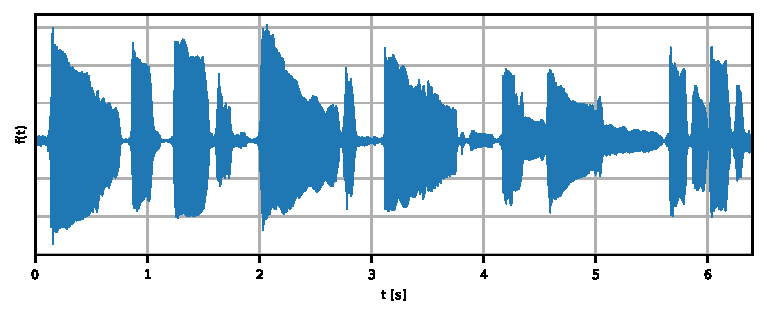
\includegraphics{papers/sonogramm/images/audioTimeDern.pdf}
    \caption{Audiospur für die Tonanalyse.
    \label{sonogramm:dernTime}
    }
\end{figure}

Eine grundsätzliche Entscheidung, die wir treffen müssen,
ist die zeitliche Auflösung, die wir haben möchten, welche 
dann auch unsere Frequenzauflösung beeinflusst.
Für unser Stück haben wir den Vorteil, dass jeweils nur einzelne
Töne gespielt werden, wir müssen also nicht zwei Töne zur selben 
Zeit erkennen.
Die benötigte Zeitauflösung können wir anhand der Geschwindigkeit des Lieds abschätzen.
Diese beträgt 83 Schläge pro Minute mit einem 4/4 Takt, also jeweils alle 0.69 Sekunden ein viertel Takt.
Möchten wir Sechzehntelnoten erkennen, darf die STFT über maximal 0.17 Sekunden
angewendet werden.
Damit die Sechzehntelnoten nicht nur in einem Segment zu sehen sind, teilen
wir die 0.17 Sekunden nochmals durch zwei.
Das liefert uns bei einer Abtastfrequenz von 44100 Hz eine ungefähre Segmentlänge von 
3800 Samples. 
Nach einem bisschen Ausprobieren ergaben sich gute Resultate bei einer Segmentlänge
von 4096 Samples.
Um die Leckfrequenzen zu unterdrücken verwenden wir ein Hammingfenster.
Somit resultiert das Sonogramm in Abbildung \ref{sonogramm:dernSono}.

Die gespielten Töne können wir nun anhand der Frequenzen 
der Peaks in den Segmenten errechnen.
Abbildung \ref{sonogramm:dernSonoPeaks} zeigt die gefundenen Frequenzen, und die
jeweiligen interessanten Abschnitte.
Die Frequenzen müssen wir nun noch in die Töne umrechnen, wobei wir jeweils auf den
nächsten Ton runden.
Wir machen die Annahme, dass der gespielte der Ton derjenige mit der höchsten Amplitude im Spektrum 
ist. 
Tabelle \ref{sonogramm:tabDern} zeigt den Vergleich mit den tatsächlich gespielten Tönen.
Diese lassen sich in diesem Fall tatsächlich gut ermitteln.
Sogar nur kurz gespielte Noten, wie das B4 im Abschnitt 10 
wurden korrekt erkannt.
Was wir vernachlässigt haben, ist der Rhythmus der gespielten Noten.
Um diesen herauszufinden, bräuchten wir jeweils die exakten Zeitpunkte, wo die Töne
beginnen und enden, was weitere Analysen erfordern würde.

\begin{figure}
    \centering
    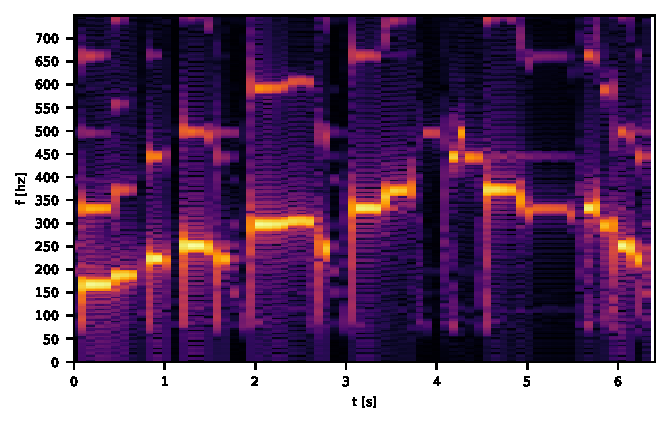
\includegraphics{papers/sonogramm/images/dernSono1.pdf}
    \caption{Sonogram des Audiosignalabschnitts. Die intensivsten Peaks der 
    jeweiligen Segmente zeigen die gespielten Grundtöne. Die weiger
    intensiven Peaks bei den n-fachen Frequenzen des Grundtones sind die Obertöne, welche durch die Physik der Saiten 
\index{Oberton}%
    entstehen.
    Ausserdem sieht man bei einigen Tönen, dass zu Beginn des Tones durch das Anspielen der Saite das Spektrum verschmiert wird
    und die eigentliche Frequenz kaum oder gar nicht erkennbar ist.
    Deshalb ist eine genügend kurze Segmentlänge nötig, damit ein Ton auf mehrere Segmente aufgeteilt wird.
    \label{sonogramm:dernSono}
    }
\end{figure}

\begin{figure}
    \centering
    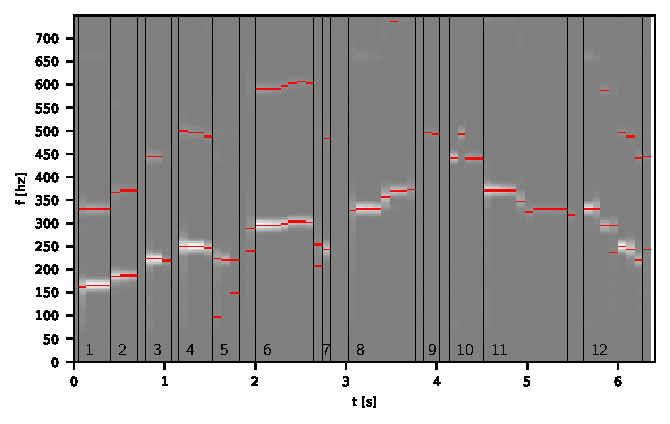
\includegraphics{papers/sonogramm/images/dernNoten.pdf}
    \caption{Gefundene Frequenzen in rot eingezeichnet. Bei gewissen 
    Segmenten werden Peaks auch bei den Frequenzen der Obertöne gefunden.
    \label{sonogramm:dernSonoPeaks}
    }
\end{figure}
	
\begin{table}
    \begin{center}
    \begin{tabular}{c | c c  } 
     \hline
     Abschnitt & Gespielte Töne & Gefundene Töne \\ [0.5ex] 
     \hline
     1 & E3 & E3 \\ 
     2 & F\musSharp3 & F\musSharp3 \\
     3 & A3 & A3 \\
     4 & B3 & B3 \\
     5 & A3 & A3 \\
     6 & D4 & D4 \\
     7 & B3  & B3 \\
     8 & \textcolor{red}{E4 slide F\musSharp4}  & \textcolor{red}{E4 - F4 - F\musSharp4} \\
     9 & B4  & B4 \\
     10 & A4 - B4 - A4   & A4 - B4 - A4 \\
     11 & \textcolor{red}{F\musSharp4 slide E4} & \textcolor{red}{F\musSharp4 - F4 - E4} \\
     12 & E4 - D3 - B3 - A3 & E4 - D3 - B3 - A3 \\
     \hline
    \end{tabular}
\end{center}
\caption{\label{sonogramm:tabDern} Vergleich der gespielten und gefundenen Töne im analysierten Abschnitt von {\em Dern Kala}.}
\end{table}
\subsection{Weitere Anwendungen}
Das Sonogramm wird in vielen Bereichen der Audioanalyse eingesetzt.
So basierten zum Beispiel frühere Spracherkennung und Sprachsynthese Methoden 
\index{Spracherkennung}%
\index{Sprachsynthese}%
auf Sonogrammen.
Nicht nur gesprochene Wörter, sondern auch Tiere wie Vögel können mit Hilfe
von Sonogrammen von ihrem Gesang bestimmt werden.
Dabei wird das Sonogramm als Input eines neuronalen Netzwerks verwendet.
\index{neuronales Netzwerk}%
Es ermöglicht mit neuronalen Netzwerken, welche für Bilder gemacht sind
Audiosignale zu analysieren.
